\chapter{文件系统、设备与交互环境}\label{chap:fs-device-shell}

文件系统、块设备、字符设备和 Shell 共同构成了用户能够直接观察到的系统环境。用户向终端输入命令后，字符设备和 TTY 层负责接收输入，Shell 解析命令并通过系统调用访问文件、创建进程或建立管道；文件读写最终通过文件系统、缓冲区和块设备到达磁盘镜像。本章只说明文件系统和 Buffer 管理在当前系统集成路径中的接口作用，不展开 inode 分配、目录项维护、缓冲区替换等细节；重点放在 RISC-V/QEMU 平台下设备模型的变化，以及 TTY 和 Shell 如何与前文的系统调用、进程管理机制连接。

\section{Unix V6 文件系统适配}

当前系统保留 Unix V6++ 的文件系统接口和主要用户态语义，包括超级块、inode、目录项、打开文件表、当前工作目录以及 \verb|open|、\verb|read|、\verb|write|、\verb|creat|、\verb|link|、\verb|unlink|、\verb|chdir|、\verb|stat|、\verb|dup| 和 \verb|pipe| 等系统调用。内核启动阶段调用 \verb|load_file_system| 读取根设备超级块，调用 \verb|init_root_directory| 取得根目录 inode，并为 0 号进程的 \verb|Userspace| 设置当前目录。随后，系统通过 \verb|kernel_open| 打开 \verb|/dev/tty1|，把文件描述符 0 和 1 绑定到控制台输入输出，为 Shell 交互建立基本环境。

相较原 \verb|main| 分支，文件系统的外部行为尽量保持稳定，资源引用方式则更偏向 Rust 的所有权模型。当前代码使用 \verb|InodeRef|、\verb|FileRef|、\verb|InodeRefGuard| 等类型封装 inode 和文件对象的引用关系，克隆引用时增加表项计数，离开作用域时通过 \verb|Drop| 归还引用。原 C++ 版本通常在调用路径中显式执行 \verb|IGet|、\verb|IPut|、\verb|CloseF| 等操作；当前版本保留这些 Unix 风格的表结构概念，并把一部分成对操作收束到引用类型的生命周期中。教学上仍可观察文件表和 inode 表，调用者忘记释放引用的机会也相应减少。

本章只说明文件系统在整机运行中的位置，不展开内部算法。进程管理模块依赖文件系统查找并读取 ELF 可执行文件，Shell 依赖目录和普通文件接口完成命令查找，管道与重定向依赖文件描述符复制和读写语义，块设备驱动则为根文件系统镜像提供持久化后端。文件系统在本文中主要作为用户程序运行环境的组成部分出现。

\begin{figure}[htbp]
  \centering
  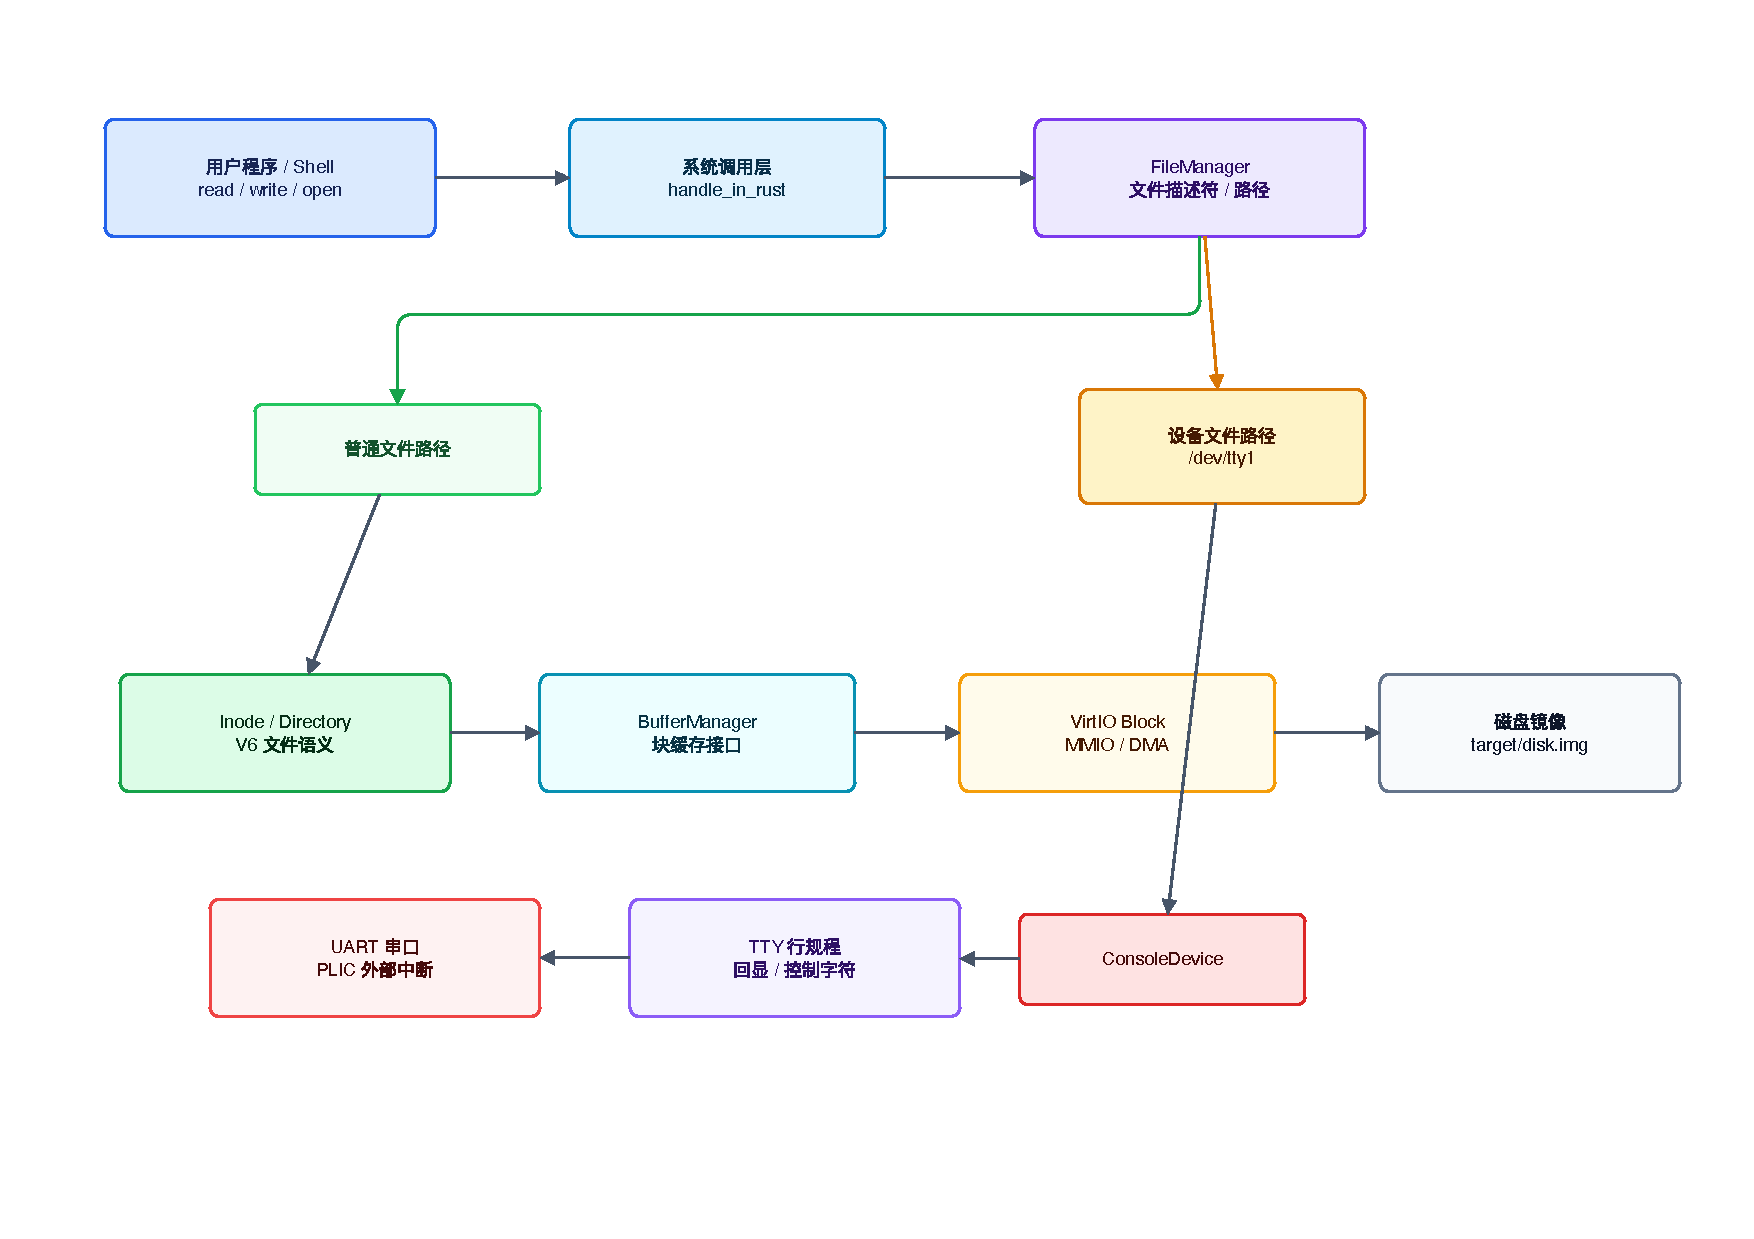
\includegraphics[width=0.95\textwidth]{figures/fs-device-path.pdf}
  \caption{文件、设备与系统调用的集成路径}\label{fig:fs-device-path}
\end{figure}

\figref{fig:fs-device-path} 展示了当前系统中普通文件和设备文件的两类访问路径。用户程序通过 C 库发起系统调用，内核在系统调用层分发到 \verb|FileManager|。目标为普通文件时，访问路径经过 inode、文件系统和 Buffer 管理，再由块设备驱动读写磁盘镜像；目标为字符设备，例如 \verb|/dev/tty1| 时，则通过设备号分发到 Console 字符设备，再进入 TTY 层。这样的分层延续了 Unix 将设备纳入文件接口的处理方式，也使 Shell 无需直接区分终端、普通文件和管道的底层实现。

\section{块设备与缓冲区接口}

原 IA-32/C++ 版本运行于 PC 机器模型，块设备主要面向 ATA/IDE 硬盘，驱动代码需要直接操作 I/O 端口、LBA28 寄存器、DMA 描述符和 8259A 中断结束命令。当前 RISC-V/Rust 版本面向 QEMU virt 机器，块设备改为 VirtIO MMIO 设备。内核通过 \verb|VirtIOBlockDriver::find_block_device| 扫描 virt 机器提供的 MMIO slot，识别 VirtIO Block 设备后建立驱动对象；读写请求通过 \verb|virtio-drivers| 库提交给设备，并以 512 字节扇区为单位访问磁盘镜像\cite{qemu_riscv_doc,virtio_1_2}。

当前系统仍保留 Unix V6++ 风格的块设备接口。\verb|BlockDevice| trait 提供 \verb|open|、\verb|close|、\verb|strategy|、\verb|start| 和 \verb|devtab| 方法，\verb|VirtIOBlockDevice| 实现该接口，并维护设备队列与活动标志。Buffer 管理器作为文件系统和块设备之间的缓冲层，负责按设备号和块号取得 \verb|Buf|，处理忙等待、延迟写、I/O 完成唤醒等流程。本节不展开缓存命中、空闲链表和写回策略，只说明它为文件系统提供统一的块读写入口。

设备适配体现了平台迁移的具体影响。旧版本依赖 x86 I/O 端口和中断控制器，设备访问与 PC 硬件细节耦合较深；当前版本使用 MMIO 地址、PLIC 外部中断和 VirtIO 标准设备，驱动路径与 QEMU virt 平台一致。VirtIO HAL 中仍需要处理 DMA 页分配、物理地址转换和共享缓冲区等底层问题，但这些内容被限制在驱动适配层中。上层文件系统继续通过 \verb|bread|、\verb|bwrite|、\verb|bdwrite| 等缓冲区接口访问块数据，磁盘后端从 ATA 迁移到 VirtIO 后，上层接口基本保持稳定。

\section{TTY 与 Shell}

字符设备是 Shell 交互的入口。当前系统用 \verb|ConsoleDevice| 实现主设备号为 0 的字符设备，并通过 \verb|console_tty| 连接到 TTY 层。读终端时，字符设备检查 TTY 输入队列是否已有完整数据；如果没有，当前进程睡眠到 TTY 的读等待通道。串口接收到输入字节后，UART 外部中断经 PLIC 进入内核，Trap 处理器读取串口数据并调用 \verb|tty_input_byte|，TTY 层完成回显、规范模式处理、退格、整行提交和读者唤醒。写终端时，输出字符经过 TTY 的输出转换，例如把换行转换为回车加换行，最终写入串口。

\begin{figure}[htbp]
  \centering
  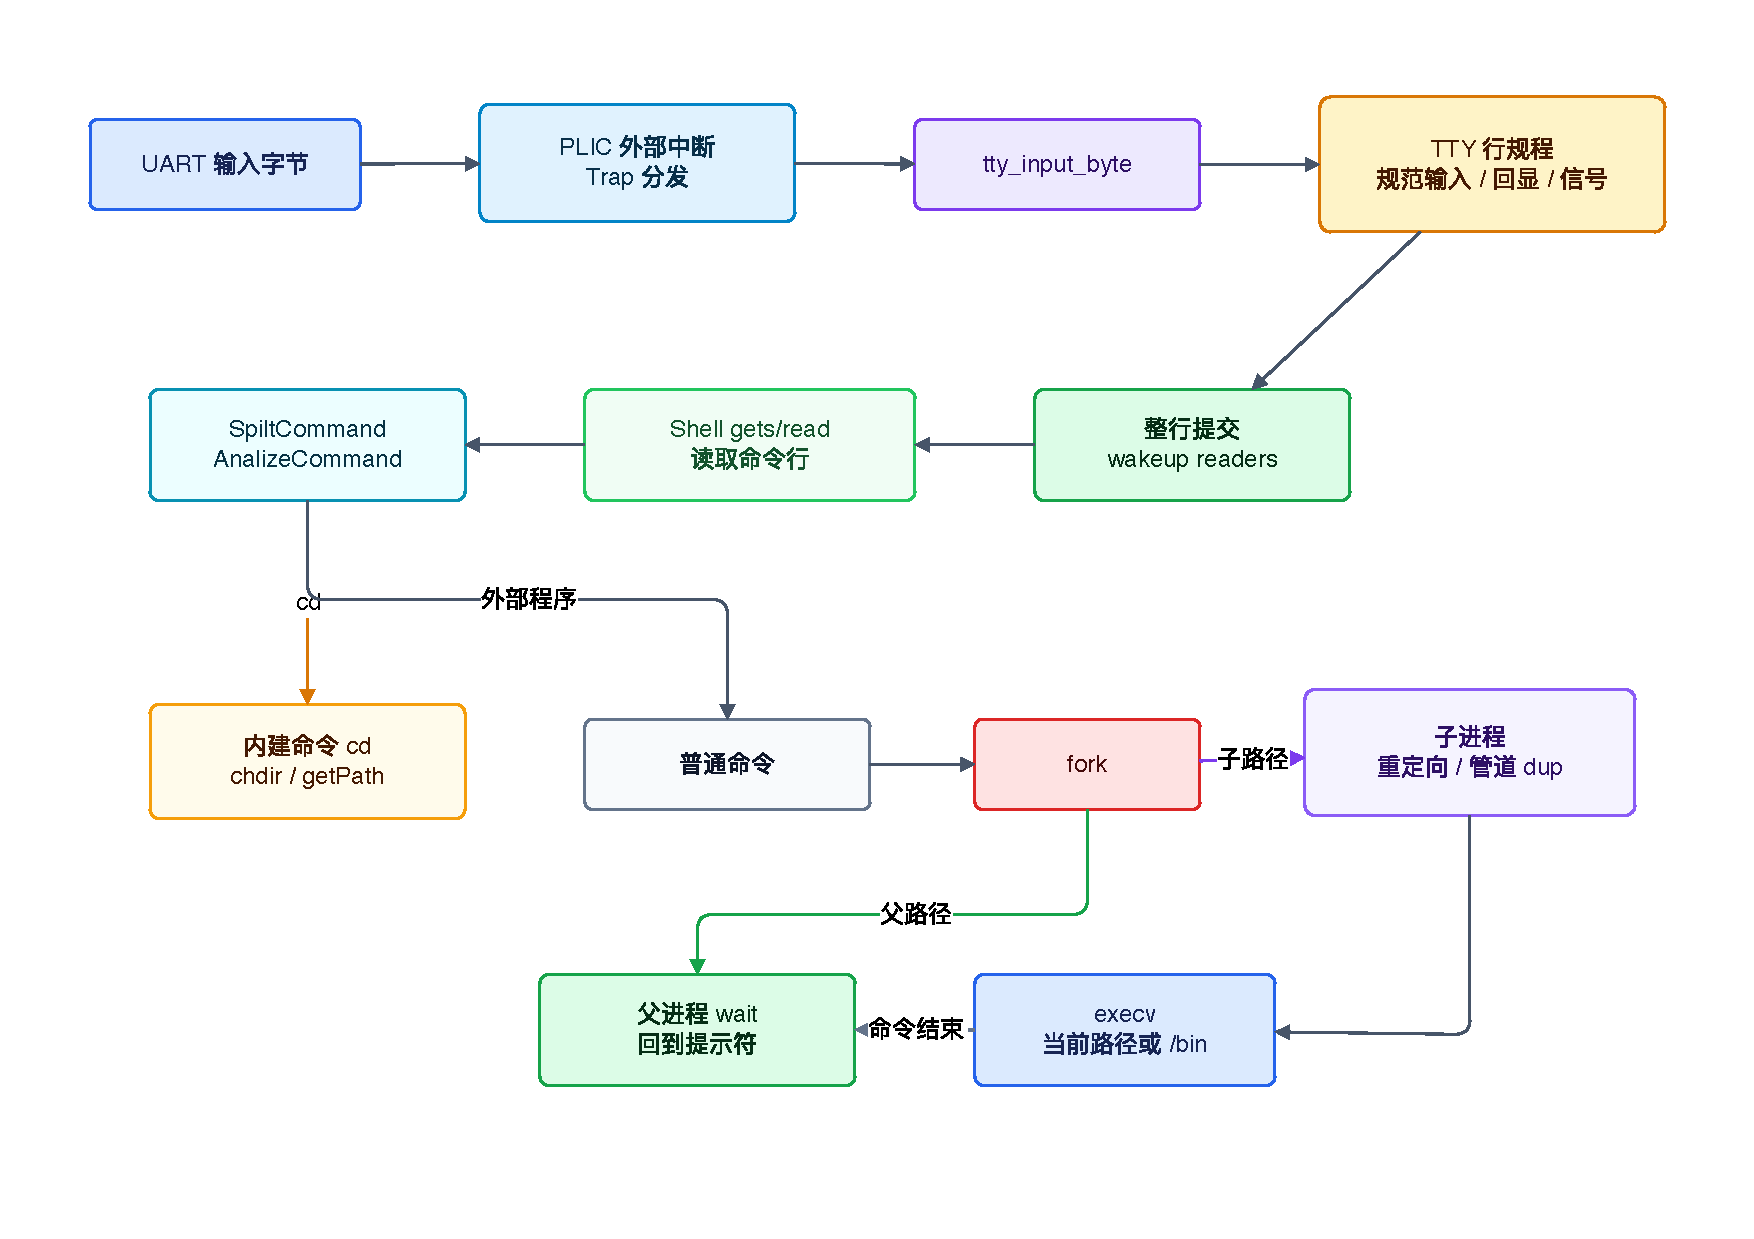
\includegraphics[width=0.95\textwidth]{figures/tty-shell-flow.pdf}
  \caption{终端输入到 Shell 执行的交互路径}\label{fig:tty-shell-flow}
\end{figure}

\figref{fig:tty-shell-flow} 展示了从输入字节到命令执行的路径。TTY 默认工作在规范输入模式，用户输入一行并按下回车后，因 \verb|read| 等待的 Shell 被唤醒。Shell 的 \verb|main1| 输出提示符，调用 \verb|gets| 读取命令行，再通过 \verb|SpiltCommand| 和 \verb|AnalizeCommand| 构造命令树。内建命令 \verb|cd| 由 Shell 直接调用 \verb|chdir| 并更新当前路径；普通命令则先 \verb|fork|，子进程完成输入输出重定向或管道描述符复制后，尝试执行当前路径下的程序，失败后再尝试 \verb|/bin| 目录下的同名程序。

当前 Shell 沿用了原 Unix V6++ 用户态 Shell 的主要结构，支持常见命令执行、管道、重定向、后台执行标志以及 \verb|shutdown|。Shell 继续使用 C 编写，并配合轻量 C 库运行；内核则以 Rust 实现。这样的安排使学生可以同时观察内核 ABI、C 运行时入口和系统调用封装之间的关系。用户程序通过 \verb|ecall| 进入内核，内核通过 RISC-V 的 \verb|a0|、\verb|a1| 等寄存器传递返回值和参数，与第 4 章的系统调用路径相互对应。

TTY 层还与信号机制相连接。当输入字符等于中断、退出或挂起控制字符时，TTY 会根据 \verb|Termios| 配置回显控制字符，并通过进程管理器向相关进程发送 \verb|SIGINT|、\verb|SIGQUIT| 或 \verb|SIGTSTP|。用户可以由此在终端中观察信号递送效果，第 7 章中的信号测试也使用这一交互入口。原 C++ 版本的 TTY 直接面向键盘和显示输出路径，当前版本把输入输出收束到 UART 串口和 Console 字符设备，更符合 QEMU virt 的无图形运行方式。
